\documentclass[journal,5pt,twocolumn]{IEEEtran}
%\makeatletter

\makeatother
\usepackage{setspace}
\usepackage{gensymb}
\usepackage{xcolor}
\usepackage{caption}
%\usepackage{stackengine}
%\usepackage{subcaption}
%\doublespacing
\usepackage{xcolor}
\usepackage{lipsum}
\singlespacing
\def\baselinestretch{1.5}
\usepackage{fancyhdr}
\pagestyle{fancy}
\fancyhf{} 

%\counterwithin{enumi}{section}
%\counterwithin{equation}{enumi}
\counterwithin{figure}{enumi}

\newcommand\figref{Fig.~\ref}
\usepackage[colorlinks=true, allcolors=black]{hyperref}

\usepackage{graphicx}
%\graphicspath{ {./images}  }
%\usepackage{amssymb}
%\usepackage{relsize}
\usepackage[cmex10]{amsmath}
\usepackage{mathtools}
%\usepackage{amsthm}
\interdisplaylinepenalty=2500
%\savesymbol{iint}
%\usepackage{txfonts}
%\restoresymbol{TXF}{iint}
\usepackage{wasysym}
\usepackage{amsthm}
\usepackage{mathrsfs}
\usepackage{txfonts}
\usepackage{stfloats}
\usepackage{cite}
\usepackage{cases}
\usepackage{mathtools}
\usepackage{subfig}
\usepackage{enumerate}	
\usepackage{enumitem}
\usepackage{amsmath}
%\usepackage{xtab}
\usepackage{longtable}
\usepackage{multirow}
%\usepackage{algorithm}
%\usepackage{algpseudocode}
\usepackage{enumitem}
\usepackage{mathtools}
%\usepackage{iithtlc}
\usepackage{tikz}
\usetikzlibrary{shapes,arrows}
%\usetikzlibrary{arrows.meta,calc,positioning}
%\usepackage[framemethod=tikz]{mdframed}
\usepackage{listings}
    \usepackage[latin1]{inputenc}                                 %%
    \usepackage{color}                                            %%
    \usepackage{array}                                            %%
    \usepackage{longtable}                                        %%
    \usepackage{calc}                                             %%
    \usepackage{multirow}                                         %%
    \usepackage{hhline}                                           %%
    \usepackage{ifthen}                                           %%
  %optionally (for landscape tables embedded in another document): %%
    \usepackage{lscape}     


%\usepackage{stmaryrd}


%\usepackage{wasysym}
%\newcounter{MYtempeqncnt}
\DeclareMathOperator*{\Res}{Res}
%\renewcommand{\baselinestretch}{4}
%\setcounter{secnumdepth}{4}
\renewcommand\thesection{\arabic{section}}
\renewcommand\thesubsection{\thesection.\arabic{subsection}}
\renewcommand\thesubsubsection{\thesubsection.\arabic{subsubsection}}
%\renewcommand\thesubsubsubsection{\thesubsubsection.\arabic{subsubsubsection}}

%\renewcommand\thesectiondis{\arabic{section}}
%\renewcommand\thesubsectiondis{\thesectiondis.\arabic{subsection}}
%\renewcommand\thesubsubsectiondis{\thesubsectiondis.\arabic{subsubsection}}
%\renewcommand\thesubsubsubsectiondis{\thesubsubsectiondis.\arabic{subsubsubsection}}
% correct bad hyphenation here
\hyphenation{Future Wireless communications}

%\lstset{
%language=C,
%frame=single, 
%breaklines=true
%}

%\lstset{
	%%basicstyle=\small\ttfamily\bfseries,
	%%numberstyle=\small\ttfamily,
	%language=Octave,
	%backgroundcolor=\color{white},
	%%frame=single,
	%%keywordstyle=\bfseries,
	%%breaklines=true,
	%%showstringspaces=false,
	%%xleftmargin=-10mm,
	%%aboveskip=-1mm,
	%%belowskip=0mm
%}

%\surroundwithmdframed[width=\columnwidth]{lstlisting}
\def\inputGnumericTable{}                                 %%

\lstset{
%language=python,
frame=single, 
breaklines=true,
columns=fullflexible
}

 \usepackage{watermark}

\begin{document}
%
\tikzstyle{block} = [rectangle, draw,
text width=7em, text centered, minimum height=4em]
\tikzstyle{sum} = [draw, circle, node distance=3cm]
\tikzstyle{input} = [coordinate]
\tikzstyle{output} = [coordinate]
\tikzstyle{pinstyle} = [pin edge={to-,thin,black}]
\tikzstyle{line} = [draw, -latex']
\theoremstyle{definition}
\newtheorem{theorem}{Theorem}[section]
\newtheorem{problem}{Problem}
\newtheorem{proposition}{Proposition}[section]
\newtheorem{lemma}{Lemma}[section]
\newtheorem{corollary}[theorem]{Corollary}
\newtheorem{example}{Example}[section]
\newtheorem{definition}{Definition}[section]
%\newtheorem{algorithm}{Algorithm}[section]
%\newtheorem{cor}{Corollary}
\newcommand{\BEQA}{\begin{eqnarray}}
\newcommand{\EEQA}{\end{eqnarray}}
\newcommand{\define}{\stackrel{\triangle}{=}}
\bibliographystyle{IEEEtran}
%\bibliographystyle{ieeetr}
\providecommand{\nCr}[2]{\,^{#1}C_{#2}} % nCr
\providecommand{\nPr}[2]{\,^{#1}P_{#2}} % nPr
\providecommand{\mbf}{\mathbf}
\providecommand{\pr}[1]{\ensuremath{\Pr\left(#1\right)}}
\providecommand{\qfunc}[1]{\ensuremath{Q\left(#1\right)}}
\providecommand{\sbrak}[1]{\ensuremath{{}\left[#1\right]}}
\providecommand{\lsbrak}[1]{\ensuremath{{}\left[#1\right.}}
\providecommand{\rsbrak}[1]{\ensuremath{{}\left.#1\right]}}
\providecommand{\brak}[1]{\ensuremath{\left(#1\right)}}
\providecommand{\lbrak}[1]{\ensuremath{\left(#1\right.}}
\providecommand{\rbrak}[1]{\ensuremath{\left.#1\right)}}
\providecommand{\cbrak}[1]{\ensuremath{\left\{#1\right\}}}
\providecommand{\lcbrak}[1]{\ensuremath{\left\{#1\right.}}
\providecommand{\rcbrak}[1]{\ensuremath{\left.#1\right\}}}
\theoremstyle{remark}
\newtheorem{rem}{Remark}
\newcommand{\sgn}{\mathop{\mathrm{sgn}}}
\providecommand{\abs}[1]{\left\vert#1\right\vert}
\providecommand{\res}[1]{\Res\displaylimits_{#1}} 
\providecommand{\norm}[1]{\lVert#1\rVert}
\providecommand{\mtx}[1]{\mathbf{#1}}
\providecommand{\mean}[1]{E\left[ #1 \right]}
\providecommand{\fourier}{\overset{\mathcal{F}}{ \rightleftharpoons}}
%\providecommand{\hilbert}{\overset{\mathcal{H}}{ \rightleftharpoons}}
\providecommand{\system}{\overset{\mathcal{H}}{ \longleftrightarrow}}
	%\newcommand{\solution}[2]{\textbf{Solution:}{#1}}
\newcommand{\solution}{\noindent \textbf{Solution: }}
\newcommand{\myvec}[1]{\ensuremath{\begin{pmatrix}#1\end{pmatrix}}}
\providecommand{\dec}[2]{\ensuremath{\overset{#1}{\underset{#2}{\gtrless}}}}
\DeclarePairedDelimiter{\ceil}{\lceil}{\rceil}
%\numberwithin{equation}{subsection}
\numberwithin{equation}{section}
%\numberwithin{problem}{subsection}
%\numberwithin{definition}{subsection}
%\makeatletter
%\@addtoreset{figure}{section}
%\makeatother
\let\StandardTheFigure\thefigure
%\renewcommand{\thefigure}{\theproblem.\arabic{figure}}
%\renewcommand{\thefigure}{\thesection}
%\numberwithin{figure}{subsection}
%\numberwithin{equation}{subsection}
%\numberwithin{equation}{section}
%\numberwithin{equation}{problem}
%\numberwithin{problem}{subsection}
%\numberwithin{problem}{section}
%%\numberwithin{definition}{subsection}
%\makeatletter
%\@addtoreset{figure}{problem}
%\makeatother
%\makeatletter
%\@addtoreset{table}{problem}
%\makeatother
\let\StandardTheFigure\thefigure
\let\StandardTheTable\thetable
\let\vec\mathbf
%%\renewcommand{\thefigure}{\theproblem.\arabic{figure}}
%\renewcommand{\thefigure}{\theproblem}
%%\numberwithin{figure}{section}
%%\numberwithin{figure}{subsection}
\def\putbox#1#2#3{\makebox[0in][l]{\makebox[#1][l]{}\raisebox{\baselineskip}[0in][0in]{\raisebox{#2}[0in][0in]{#3}}}}
     \def\rightbox#1{\makebox[0in][r]{#1}}
     \def\centbox#1{\makebox[0in]{#1}}
     \def\topbox#1{\raisebox{-\baselineskip}[0in][0in]{#1}}
     \def\midbox#1{\raisebox{-0.5\baselineskip}[0in][0in]{#1}}
\title{ 
%	\logo{
BANDWIDTH CALCULATION
%	}
}
\author{ Under guidance of Dr. GVV SHARMA}% <-this % stops a space
\thiswatermark{\centering \put(-50,-105){
\includegraphics[scale=0.5]{iith.png}}}
% make the title area
\maketitle
\tableofcontents
\section{\textbf{Introduction}}
Bandwidth is an important concept in signal processing and communication engineering.
The main objective is to analyze an audio signal ,to plot the magnitude spectrum of the audio signal and calculate its bandwidth using power spectral density.\\
\section{\textbf{Bandwidth Calculation}}
\subsection{\textbf{Bandwidth calculation method}}

Bandwidth refers to the range of frequencies over which a signal or system operates. There are several methods to calculate the bandwidth of a signal, including the 3dB attenuation method and the spectral density method.\\
\begin{enumerate}
\item  The 3dB attenuation method involves finding the frequency range where the signal's power or amplitude is reduced by half (-3dB) from its maximum value.However, it does not take into account the full frequency spectrum of the signal or system, and may not accurately reflect the actual bandwidth of the signal.
\item The spectral density method calculates the bandwidth of a signal or system by analyzing its frequency content. Specifically, it calculates the power spectral density (PSD) of the signal or system, which is a measure of how the power of the signal is distributed across different frequencies. The bandwidth is then defined as the frequency range over which 99\%of the total power is contained.\\
 This method provides a more accurate and comprehensive measure of bandwidth as it takes into account the entire frequency spectrum of the signal or system.
\end{enumerate}

\subsection{\textbf{Steps for calculating the bandwidth of the signal}}
   

\begin{enumerate}
\item Loading the Audio File:  loading the audio file using the wavfile.read() function from the scipy.io.wavfile module. This returns the sampling frequency and the audio data 

\item Computing the Fourier Transform:The FFT is performed on the audio signal using np.fft.fft() function.This transforms the audio data from the time domain to the frequency domain.
\begin{align}
X(f) = FFT(x(t))
\end{align}

\item Calculating the frequency Range: The frequency range is calculated using np.fft.fftfreq() function . This function calculates the frequencies for each sample in the audio signal. The frequency range is used to plot the magnitude spectrum of the audio signal.

\item Calculating the Power Spectral Density: PSD is the power of the signal per unit of frequency. The PSD is calculated by squaring the absolute value of the FFT.
\begin{align}
S(f)=\lvert X(f) \rvert^2 
\end{align}

\item Finding the Frequency Range with Significant Power:
To calculate the bandwidth of the signal,  find the range of frequencies with significant power. We can do this by setting a threshold on the PSD and identifying the frequencies that exceed this threshold.set the threshold to 0.1 times the maximum PSD value.
\item Calculating the Bandwidth: Calculate the bandwidth as the difference between the maximum and minimum frequencies in the range with significant power.
\end{enumerate}

\section{\textbf{Result}}
Analyzes the audio signal and plots its magnitude spectrum. The bandwidth of the audio signal is a calculated using power spectral density. Obtain the bandwidth of the audio as 2 khz.The spectrum of input audio signal is plotted in \figref{fig:input_spectrum} using below code
\begin{center}
\fcolorbox{red}{white}{\parbox{12.5cm}
{\href{https://github.com/Gangagopinath/fwc/tree/main/FM/code}
{/codes/input.py}}}
\end{center}

\begin{figure}
\centering 
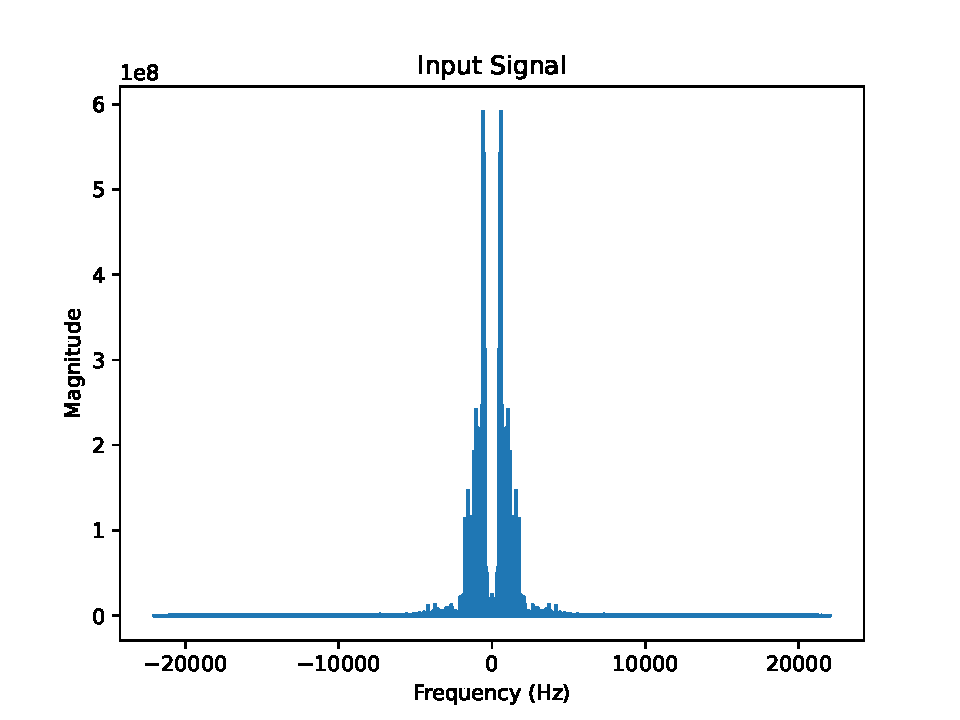
\includegraphics[width=\columnwidth]{./inputs.pdf}
\caption{spectrum analysis of input signal}
\label{fig:input_spectrum}
\end{figure}



\end{document}